%-----------------------------------------------------------------------------------------------
\makeatletter
\immediate\write18{datelog > \jobname.info} % site script for $(date '+%Y-%m-%d %Hh%Mm%Ss')
\makeatother
%-----------------------------------------------------------------------------------------------
\usetheme{Copenhagen}
\usepackage{beamercolorthemeUTF2}
\usefonttheme{serif}
%-----------------------------------------------------------------------------------------------
\usepackage[utf8]{inputenc}
\usepackage[english,brazil]{babel} % last becomes the active one
\usepackage{pslatex}
\usepackage{amssymb,amsmath}
\usepackage{soul}
\usepackage[squaren,Gray]{SIunits}
\usepackage{xspace}
%-----------------------------------------------------------------------------------------------
\definecolor{enfa}{rgb}{0.90,0.30,0.30} % Emphasis
%-----------------------------------------------------------------------------------------------
\newcommand{\enfa}[1]{{\color{enfa}{#1}}}
\newcommand{\gray}[1]{{\color{gray}{#1}}}
\newcommand{\txtpic}[1]{%
    \fcolorbox{lightgray}{white!90!black}{{#1}} 
}
%-----------------------------------------------------------------------------------------------
\newcommand{\vet}[1]{\underline{{#1}}}
\newcommand{\mat}[1]{\underline{\underline{{#1}}}}
\newcommand{\cub}[1]{\underline{\underline{\underline{{#1}}}}}
\newcommand{\eqdef}{{\ensuremath\stackrel{\text{\tiny def}}{=}}}
%-----------------------------------------------------------------------------------------------
\newcommand{\BkgImgH}[1]{% Places an image centered on the slide background filling the height
    \usebackgroundtemplate{\parbox{\paperwidth}{%
        \vspace*{1sp}\centering\includegraphics[height=\paperheight]{{#1}}
}}}
\newcommand{\BkgImgW}[1]{% Places an image centered on the slide background filling the width
    \usebackgroundtemplate{\parbox{\paperwidth}{%
        \vspace*{1sp}\centering\includegraphics[width=\paperwidth]{{#1}}
}}}
\newcommand{\ArtEndH}[3]{% Transitions to plain image (last) slide: #1:prefix #2,#3:extensions
    \BkgImgH{root/../art/#1.#2}
    \frame[plain]{\transdissolve\vspace*{80mm}\color{white}\bf\input{root/../art/#1.#3}}
}
\newcommand{\ArtEndW}[3]{% Transitions to plain image (last) slide: #1:prefix #2,#3:extensions
    \BkgImgW{root/../art/#1.#2}
    \frame[plain]{\transdissolve\vspace*{80mm}\color{white}\bf\input{root/../art/#1.#3}}
}
\newcommand{\ImgColW}[3]{% Inserts a full-width image in a column
    \includegraphics[width=\columnwidth]{root/../art/#1.#2}\\[-0.6em]
    \parbox{\columnwidth}{\tiny\hfill\input{root/../art/#1.#3}}
}
%-----------------------------------------------------------------------------------------------
\title{A.03.01 -- Trabalho de Fronteira}
\subtitle{(Sistemas Fechados)}
\author{Prof.~C.~Naaktgeboren, PhD}
\date{%
    \texttt{Compiled on \input{\jobname.info}}\\[\medskipamount]
    
\includegraphics[height=6.0mm]{root/00-res/cc/by-nc-nd-88x31.pdf}
}
%-----------------------------------------------------------------------------------------------
\begin{document}
%-----------------------------------------------------------------------------------------------
\logo{%
    \parbox{126mm}{% There's a 1mm gap on each side of the 128mm x 96mm slide logo line
        
\includegraphics[height=6.0mm]{root/00-res/UTFPR/UTFPR-logo-A.pdf}\hfill%
        
\includegraphics[height=6.0mm]{root/00-res/logo/CNThermSci-logo-A.pdf}%
}} % Alpha logos
%-----------------------------------------------------------------------------------------------
%{%
%    \usebackgroundtemplate{%
%        \parbox{\paperwidth}{%
%            \vspace*{1sp}\centering\includegraphics[height=\paperheight]%
%                {art/landscape-615428_1280.jpg}
%    }}
    \frame{\titlepage}
%}
%-----------------------------------------------------------------------------------------------
%{%
%    \usebackgroundtemplate{%
%         \parbox{\paperwidth}{%
%             \vspace*{1sp}\centering\includegraphics[height=\paperheight]%
%                 {art/mountains-landscape-1149580_1280.jpg}
%    }}
%    \frame{\tableofcontents}
%}
%-----------------------------------------------------------------------------------------------
\section{Trabalho de Fronteira}

\subsection{Qualitativo}

    % !j 96 -i8
    %-------------------------------------------------------------------------------------------
    \begin{frame}{Trabalho de Fronteira -- Definição}\vspace*{-2em}
        \begin{columns}
        \column{0.70\textwidth}
        Trabalho de fronteira, $W_f$ (\kilo\joule)                          \\[\medskipamount]
        \begin{itemize}
            \item É a \alert{interação  energética}                         \\[\medskipamount]
            \item de um \enfa{sistema compressível simples}                 \\[\medskipamount]
            \item capaz de \enfa{diretamente} realizar                      \\[\medskipamount]
            \item \enfa{trabalho mecânico}                                  \\[\medskipamount]
            \item por meio de uma \enfa{fronteira móvel}.
        \end{itemize}
        \column{0.30\textwidth}
        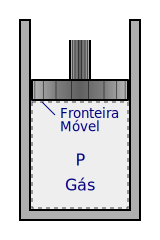
\includegraphics[width=\columnwidth]{fig/A0301-pt-VPistCyl.pdf}
        \end{columns}
    \end{frame}
    %-------------------------------------------------------------------------------------------

    % !j 96 -i8
    %-------------------------------------------------------------------------------------------
    \begin{frame}{Trabalho de Fronteira -- Aplicações}\vspace*{-2em}
        \begin{columns}
        \column{0.55\textwidth}
        Aplicações incluem:                                             \\[\medskipamount]
        \begin{itemize}
            \item Motores de combustão interna                          \\[\medskipamount]
            \item Motores \bf\alt<1>{\enfa{Stirling}}{Stirling}\rm      \\[\medskipamount]
            \item Compressores alternativos                             \\[\medskipamount]
            \item Motores \bf\alt<2>{\enfa{lineares}}{lineares}\rm      \\[\medskipamount]
            \item Elevadores de carga e atuadores                       \\[\medskipamount]
            \item Expansores \bf\alt<3>{\enfa{criogênicos}}{criogênicos}\rm
        \end{itemize}
        \column{0.45\textwidth}
            \only<1>{\ImgColW{EuroDishSBP_front}{jpg}{txt}}
            \only<2>{\ImgColW{vintage-4273640_1280}{jpg}{txt}}
            \only<3>{\ImgColW{6350734512_4ca40e0711_o}{jpg}{txt}}
        \end{columns}
    \end{frame}
    %-------------------------------------------------------------------------------------------

\subsection{Quantitativo}

    % !j 96 -i8
    %-------------------------------------------------------------------------------------------
    \begin{frame}{Trabalho de Fronteira -- Em Termos de Propriedades}\vspace*{-2em}
        \uncover<1->{$$\delta{W_f} \equiv \vec{F} \cdot d\vec\ell \rightharpoondown$$}
        \uncover<2->{$$\delta{W_f} = \frac{F}{A} d\ell{A} \rightharpoondown$$}
        \uncover<3->{$$\delta{W_f} = PdV$$}
        \begin{figure}
            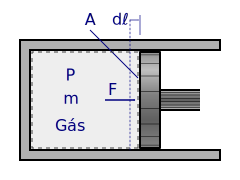
\includegraphics[width=5.0cm]{fig/A0301-pt-HPistCyl.pdf}
        \end{figure}
    \end{frame}
    %-------------------------------------------------------------------------------------------

    % !j 96 -i8
    %-------------------------------------------------------------------------------------------
    \frame{
        \frametitle{Trabalho de Fronteira}\vspace*{-2em}

       \begin{figure}
            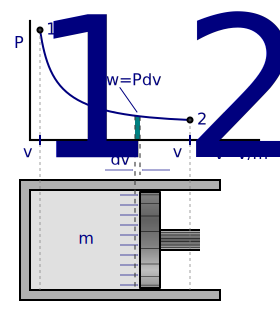
\includegraphics[width=5.0cm]{fig/A0301-pt-HPistCylPlot.pdf}
        \end{figure}

    }
    %-------------------------------------------------------------------------------------------

    % !j 96 -i8
    %-------------------------------------------------------------------------------------------
    \begin{frame}{Trabalho de Fronteira -- Teorema}\vspace*{-2em}
        \framesubtitle{Here's a subtitle}
        \begin{theorem}
            Colors do mix.
        \end{theorem}
        \begin{proof}
            It's all over this presentation!
        \end{proof}
    \end{frame}
    %-------------------------------------------------------------------------------------------


\section{Tópicos de Leitura}

    %------------------------------------------------------------------------------------------
    \begin{frame}[allowframebreaks]{Tópicos de Leitura}
        \begin{thebibliography}{Çengel, Y.~A., 2013}
            \bibitem[Çengel, Y.~A., 2013]{2013-CengelYA+BolesMA-AMGH}
                Çengel, Y.~A. e Boles, M.~A.
                \newblock{{\em Termodinâmica $7^\mathrm{a}\!$ Edição\/}. \enfa{Seção~4-1.}}
                \newblock{\footnotesize AMGH. Porto Alegre. ISBN 978-85-8055-200-3.}
        \end{thebibliography}
    \end{frame}
    %------------------------------------------------------------------------------------------

    % Finishes with stunning image, with credit
    \ArtEndH{italy-1587287_1280}{jpg}{txt}

%-----------------------------------------------------------------------------------------------
\end{document}
%-----------------------------------------------------------------------------------------------

